% sec1_method.tex — 第1节 方法
\section{方法}

% 本节介绍研究背景与所提改动方案。

\subsection{研究背景与问题}

3D Gaussian Splatting（3DGS）\cite{kerbl20233d} 以显式高斯基元为场景表示，
通过可微光栅化实现了高质量的实时渲染与快速训练。然而，原始 3DGS 产生的高斯集合
无组织、不具备拓扑结构，难以直接提取用于下游任务（物理仿真、编辑、3D 打印等）的
表面网格（Mesh）。
SuGaR（Surface-Aligned Gaussian Splatting）\cite{guedon2024sugar} 通过表面对齐
正则化策略，鼓励高斯基元贴合真实表面、协方差沿表面方向压缩，再借助 Poisson
表面重建从对齐后的高斯中提取三角网格。

本工作围绕三个核心问题展开：
\begin{enumerate}[label=(\arabic*)]
  \item 能否在有限预算（3DGS $\leq$ 7k 迭代，Coarse SuGaR $\leq$ 15k 迭代）下
        从零跑通完整的 3DGS $\to$ Coarse SuGaR $\to$ Mesh 提取流程？
  \item 能否提出一项进入训练或提取主流程的代码改动，并通过对照实验验证其效果？
  \item 改动是否带来了可观察的几何或渲染质量差异？若无，原因何在？
\end{enumerate}

\subsection{改动方案：Poisson 前的多视角深度一致性剔点}
\label{subsec:modification}

图~\ref{fig:pipeline} 给出了完整流程的全局视图，蓝色框为本文新增模块。

\begin{figure}[htbp]
  \centering
  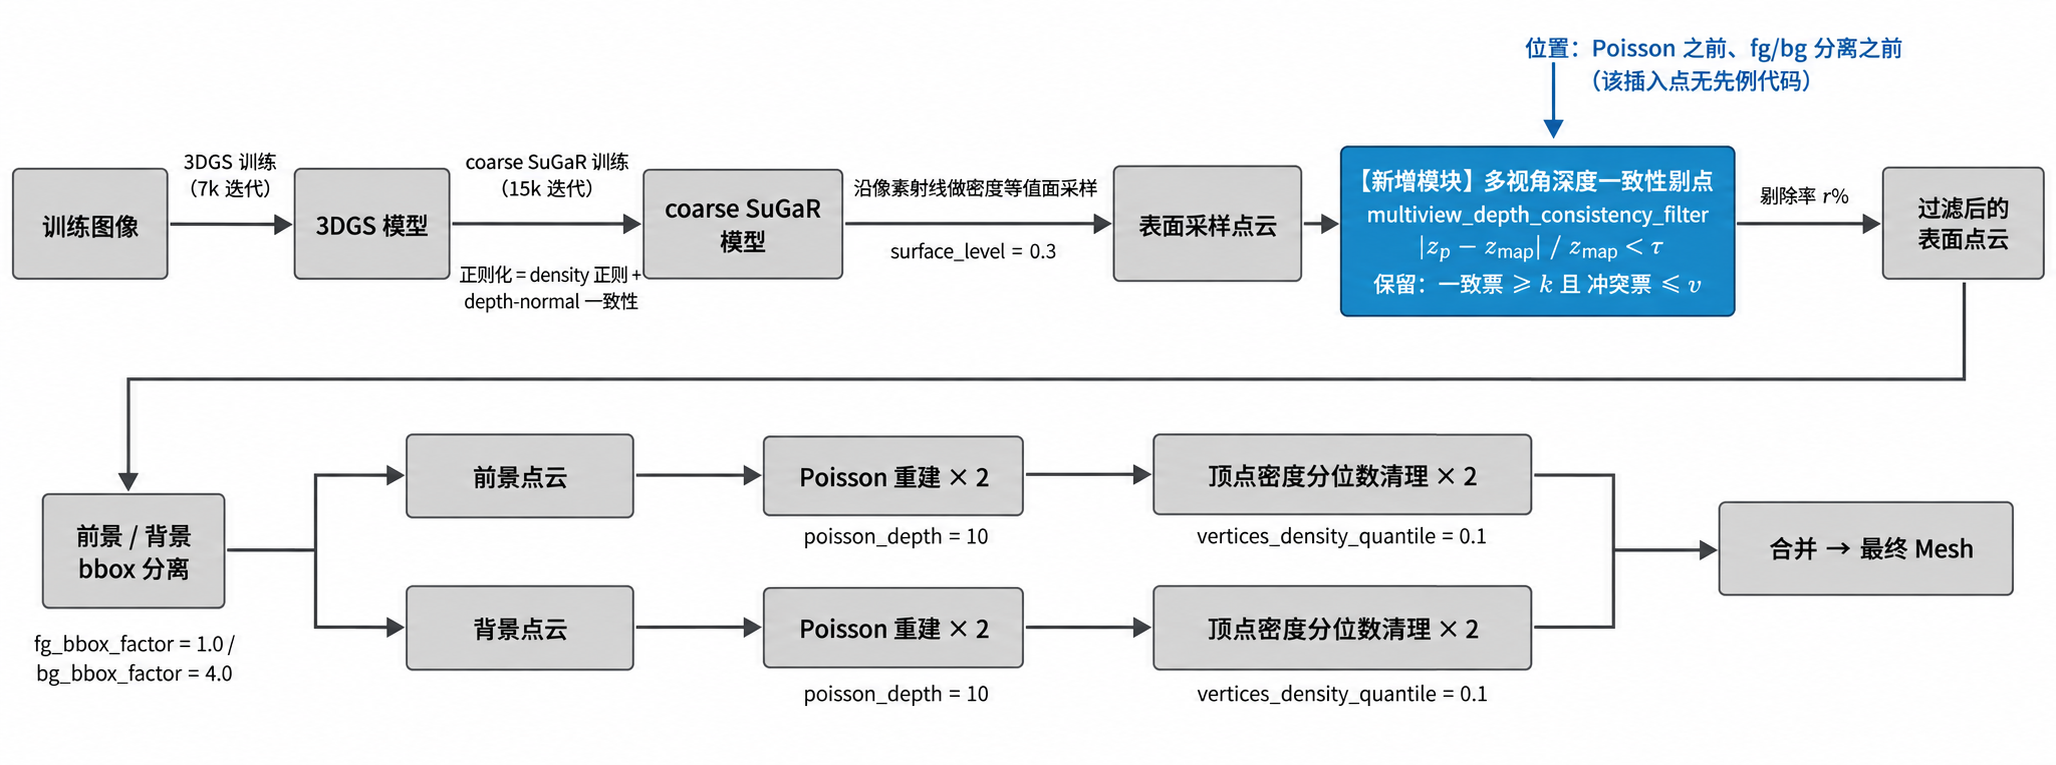
\includegraphics[width=\textwidth]{figures/改动示意图_A_流程.png}
  \caption{SuGaR Mesh 提取完整流程图。
  灰色节点为原始 SuGaR 流程，蓝色框为本文新增的多视角深度一致性剔点模块，
  插入位置为表面点采样之后、前景/背景分离与 Poisson 重建之前。}
  \label{fig:pipeline}
\end{figure}

%% ---------- 1.3.2 问题与动机 ----------
\subsubsection{问题与动机}
\label{sssec:motivation}

SuGaR \cite{guedon2024sugar} 的表面采样步骤在每个训练视角\emph{独立}进行：
沿该视角的射线找到密度等值面后即记录为表面点。
这种逐视角采样机制保证了每个点在其\emph{生成视角}下具有自洽的深度与法向，
但跨视角来看，某些采样点实际上悬浮在自由空间中——
它们对应的密度峰值只在单一视角的射线方向上存在，
并不被其他训练视角观测所支持。

这类\textbf{单视角自洽但跨视角不一致}的表面点主要产生两种伪影：
\begin{itemize}
  \item \textbf{漂浮几何}（floaters）：
        散布在场景空域中的孤立点簇，进入 Poisson 后形成
        膜状伪表面与薄壳连接；
  \item \textbf{背景壳}（background shells）：
        在远景区域（如天空、远处建筑面）由单色区域的密度累积产生的
        大面积伪表面，常表现为包裹整个场景的薄壳。
\end{itemize}

SuGaR 现有的两道后处理——统计离群点移除
与 Poisson 顶点密度分位数裁剪——
均基于局部几何统计，无法有效识别上述在几何分布上并不异常、
但在多视角一致性上不成立的虚假表面点。
图~\ref{fig:before-after} 以示意方式展示了剔点前后表面点云与 Poisson Mesh 的对比。

\begin{figure}[htbp]
  \centering
  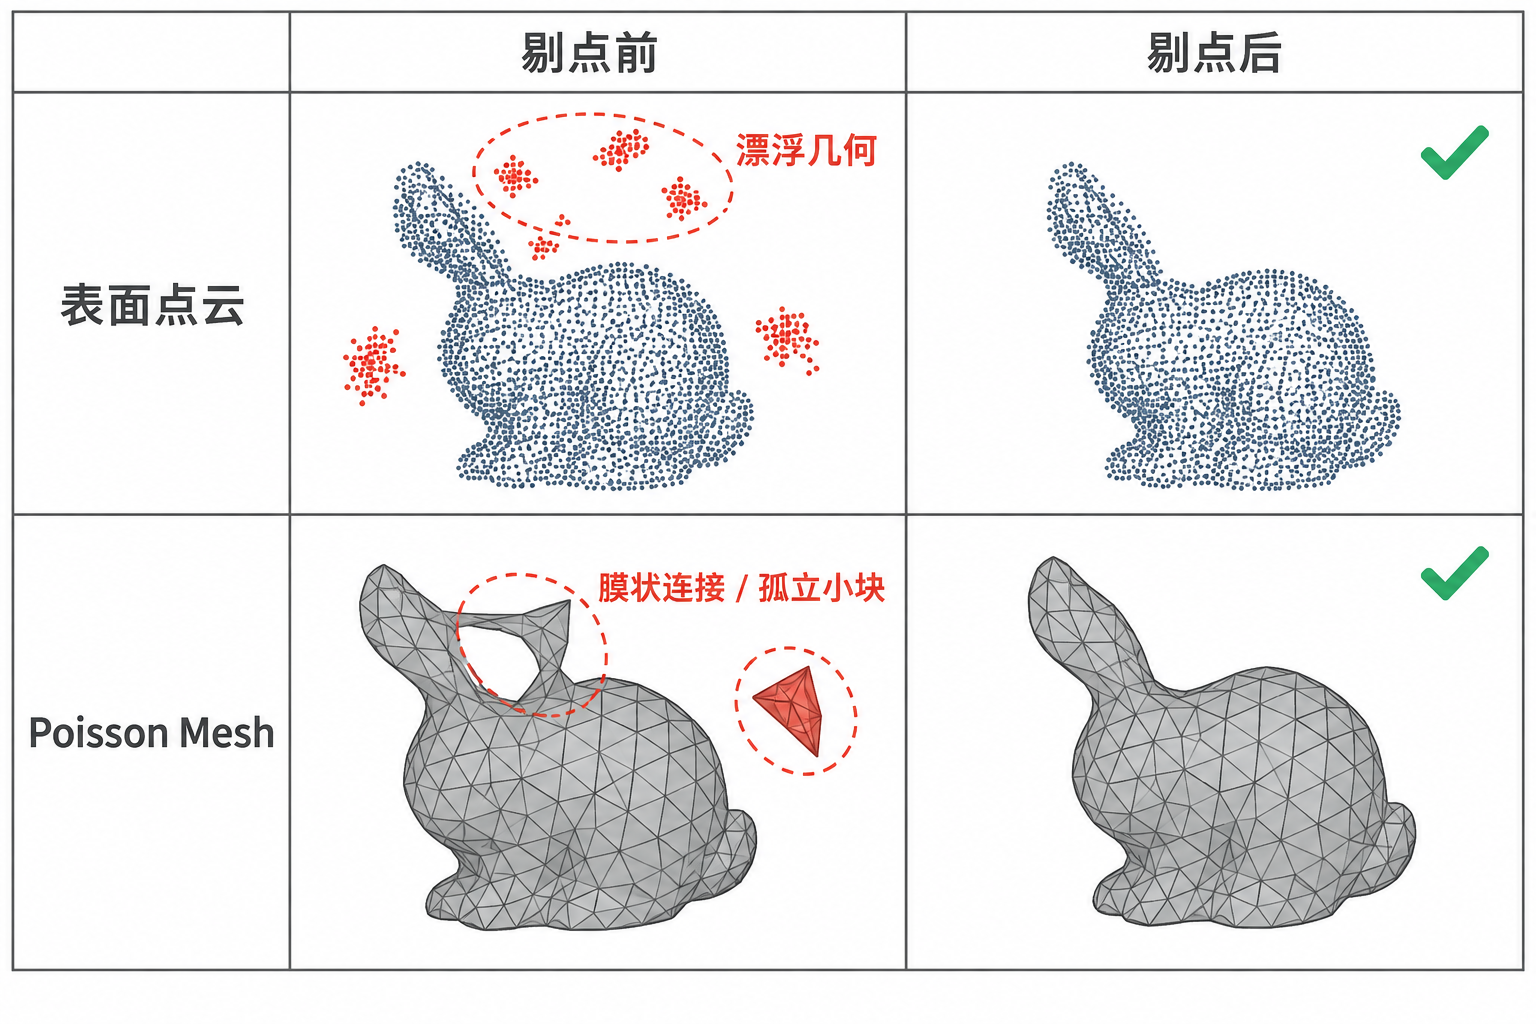
\includegraphics[width=0.85\textwidth]{figures/改动示意图_C_前后对比.png}
  \caption{剔点前后对比示意。
  上排：表面点云，剔点前含明显漂浮几何（红色标注），剔点后更干净。
  下排：Poisson Mesh，剔点前存在膜状连接与孤立小块，剔点后网格更紧凑。}
  \label{fig:before-after}
\end{figure}

%% ---------- 1.3.3 方法描述 ----------
\subsubsection{方法描述}
\label{sssec:method-detail}

\paragraph{符号定义。}
设 Coarse SuGaR 训练完成后，对某一 \texttt{surface\_level}
值采样得到的表面点集合为 $\mathcal{P} = \{p_i\}_{i=1}^{N}$，
训练相机集合为 $\mathcal{C} = \{c_j\}_{j=1}^{|\mathcal{C}|}$。
从 $\mathcal{C}$ 中均匀抽取 $M$ 个相机（固定 \texttt{seed}=0）
组成参考相机子集 $\mathcal{C}_M$。
对 $\mathcal{C}_M$ 中的每个相机 $c_j$，
预先用 SuGaR 的 \texttt{render\_depth\_and\_normal} 缓存其渲染深度图
$D_j \in \mathbb{R}^{H \times W}$。

\paragraph{判据。}
对点 $p_i$，将其投影到相机 $c_j$ 得到像素坐标 $(u, v)$ 与相机空间深度 $z_p$。
取深度图对应像素值 $z_{\mathrm{map}} = D_j(u, v)$。
定义以下三种投票：

\begin{itemize}
  \item \textbf{一致票}（consistent vote）：
        $|z_p - z_{\mathrm{map}}| < \tau \cdot z_{\mathrm{map}}$，
        即相对深度差在容差 $\tau$ 以内；
  \item \textbf{空域冲突票}（free-space conflict vote）：
        $z_p < z_{\mathrm{map}} - \tau \cdot z_{\mathrm{map}}$，
        即点明显浮在该视角已知表面\textbf{之前}的自由空间中；
  \item \textbf{无效}（不计票）：
        点落在相机 $c_j$ 视锥之外，或深度图对应像素无有效深度值。
\end{itemize}

\paragraph{保留条件。}
点 $p_i$ 被保留当且仅当同时满足：
\begin{equation}
  \label{eq:keep-condition}
  \underbrace{\sum_{j \in \mathcal{C}_M} \mathbf{1}[\text{一致}(p_i, c_j)]}_{\text{一致票数}} \;\geq\; k_{\min}
  \quad \text{且} \quad
  \underbrace{\sum_{j \in \mathcal{C}_M} \mathbf{1}[\text{冲突}(p_i, c_j)]}_{\text{冲突票数}} \;\leq\; v_{\max}
\end{equation}
其中 $k_{\min}$ 默认为2，
$v_{\max}$ 默认为1。
图~\ref{fig:vote-criterion} 以两个典型案例直观展示了投票判据的工作方式。

\begin{figure}[htbp]
  \centering
  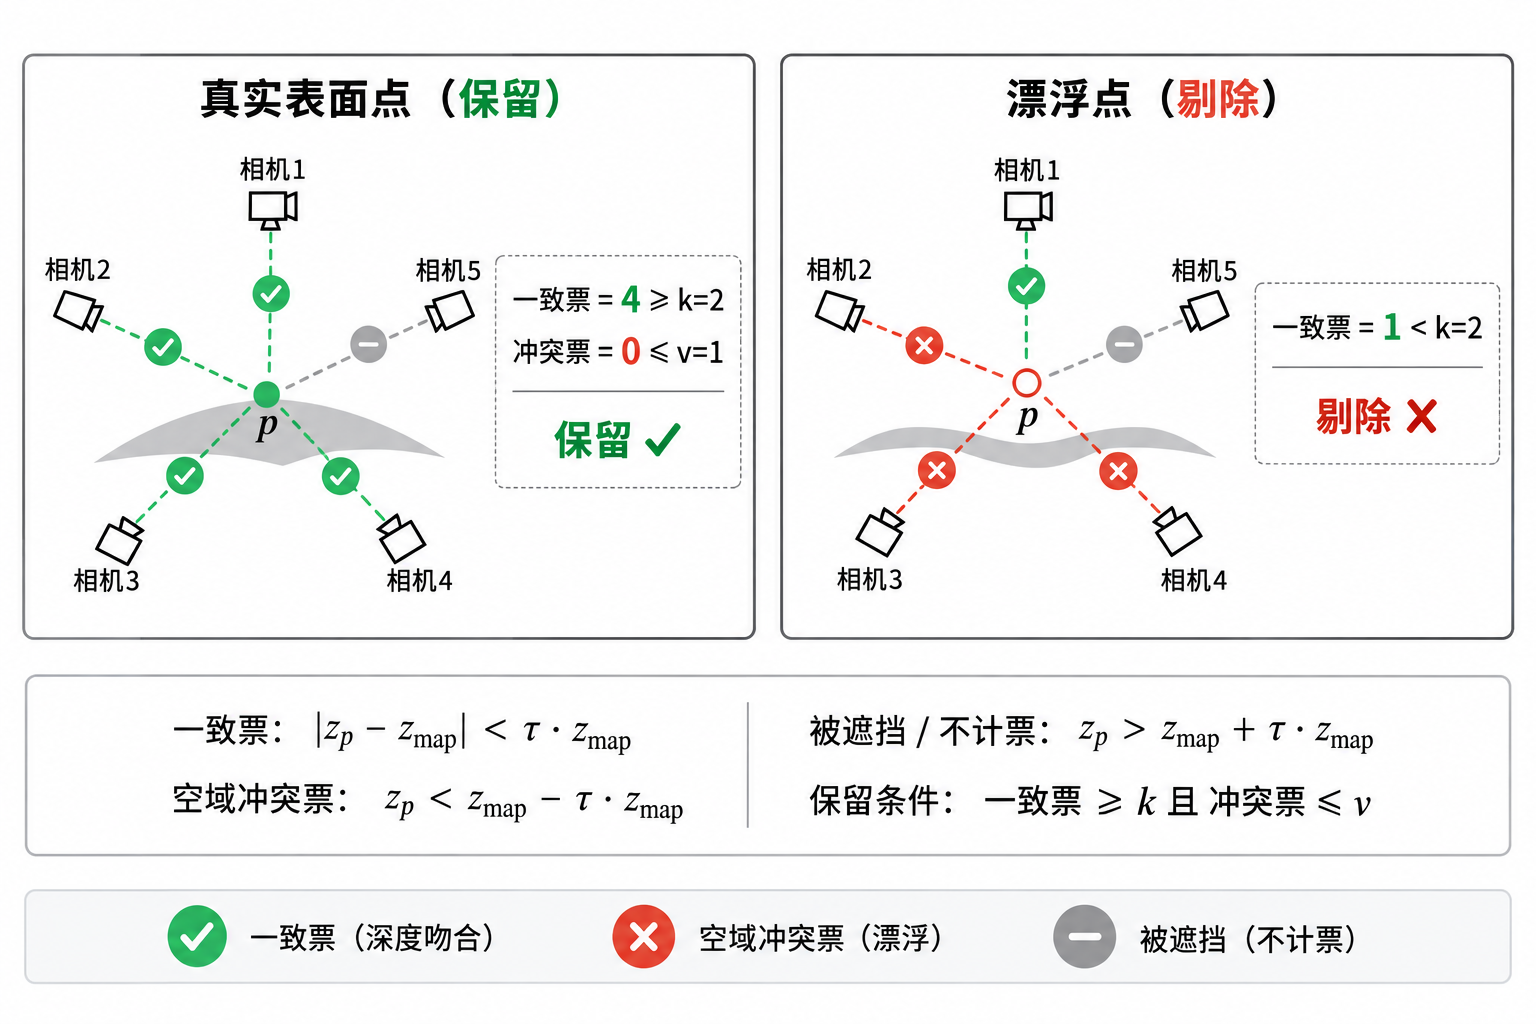
\includegraphics[width=0.9\textwidth]{figures/改动示意图_B_判据.png}
  \caption{多视角深度一致性投票判据示意。
  左：真实表面点获得 4 个一致票，满足保留条件（一致票 $\geq k{=}2$ 且冲突票 $\leq v{=}1$）。
  右：漂浮点仅获 1 个一致票且有 3 个冲突票，被剔除。
  绿色为一致票（深度吻合），红色为空域冲突票（漂浮），灰色为被遮挡（不计票）。}
  \label{fig:vote-criterion}
\end{figure}

全部超参数及默认值见附录表~\ref{tab:mv-hyperparams}，
其中 $\tau$ 为主要消融变量，扫描范围 $\{0.01, 0.02, 0.05\}$。
完整算法伪代码见附录算法~\ref{alg:mv-filter}。

